% !TEX TS-program = pdflatex
% !TEX root = ../tesi.tex

%************************************************
\chapter{AMBIENTAZIONE IN UNITY}
\label{chp:Ambientazione in Unity}
%************************************************

\section{Descrizione dell'ambientazione}

Come motore grafico è stato scelto quello di Unity, tra i più usati in ambito videoludico, per poter rappresentare l'idea visiva alla base
della composizione ideata.
L'Ambientazione scelta è quella di un ospedale psichiatrico abbandonato circondato da un'oscura foresta, che è classica scelta tra le ambientazioni dei generi Horror dei videogiochi e nei
film.\\
La scenografia prende spunto dal titolo, in quanto, un personaggio ci fa vedere attraverso i suoi occhi un ambiente tetro, privo
di illuminazione, non permettendoci di vedere al meglio ciò che ci circonda, inducendo ansia, illusioni ottiche e acustiche dettate da 
un'entità soprannaturale.
\\

\subsection*{Catture Grafiche}

\begin{figure}[h]
    \centering
    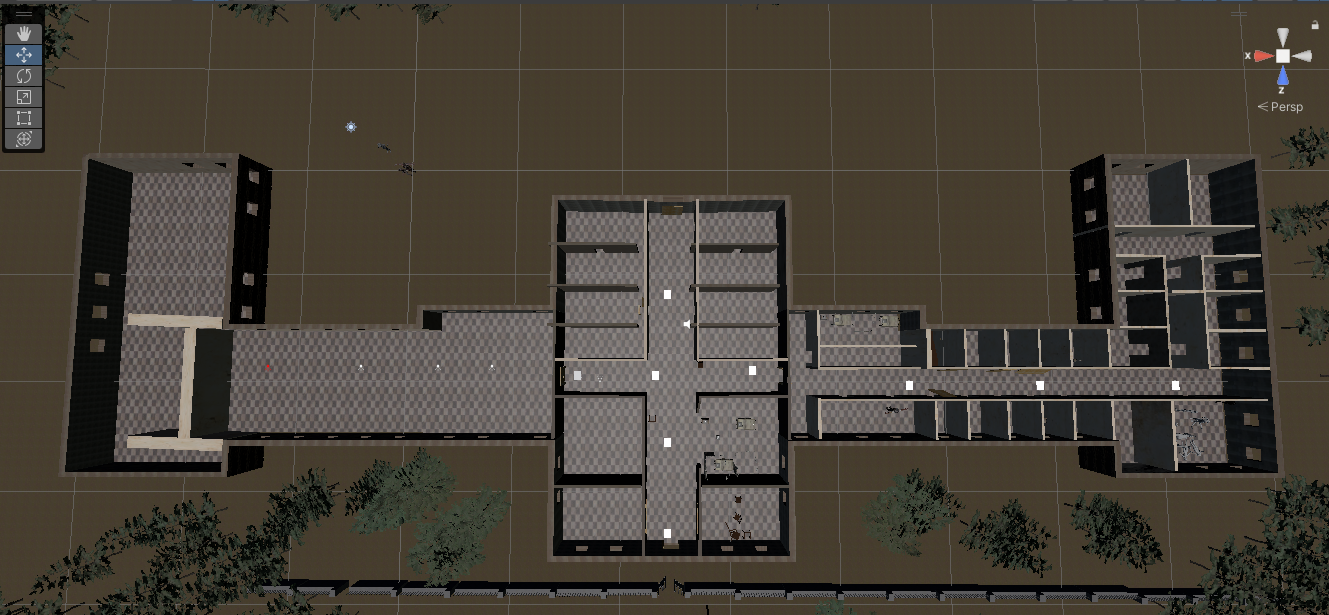
\includegraphics[width=1.2\textwidth]{piantina.png}
    \caption{⟨Piantina dell'ambientazione grafica⟩}
    \label{fig:⟨etichetta⟩}
    \end{figure}

    \begin{figure}[h]
        \centering
        \includegraphics[width=1.2\textwidth]{fronte manicomio.png}
        \caption{⟨Fronte dell'ambientazione grafica⟩}
        \label{fig:⟨etichetta⟩}
        \end{figure}

        \begin{figure}[h]
            \centering
            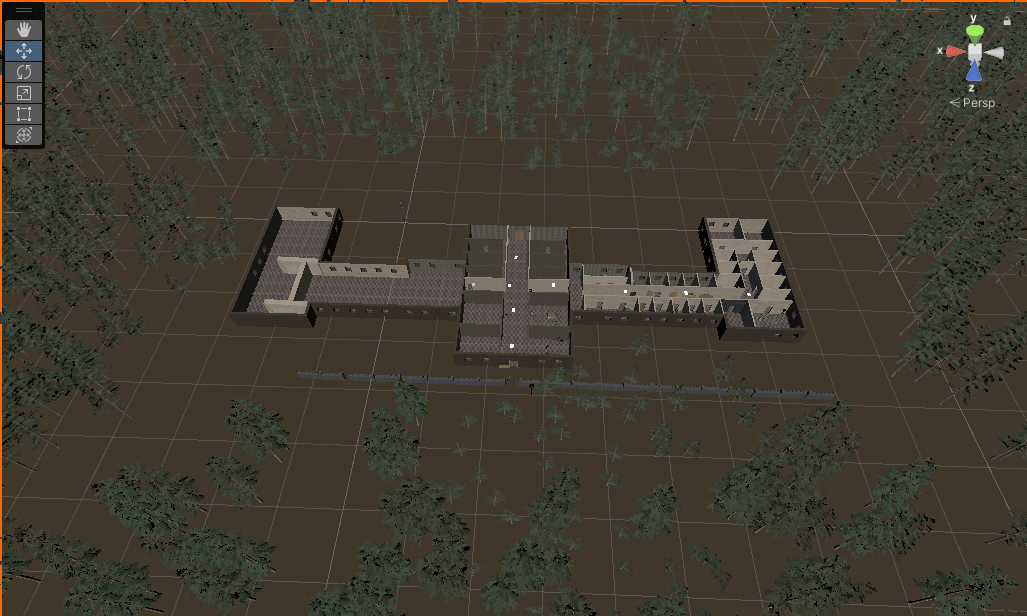
\includegraphics[width=1.2\textwidth]{landscape manicomio.png}
            \caption{⟨Panoramica dell'ambientazione grafica⟩}
            \label{fig:⟨etichetta⟩}
            \end{figure}